


\documentclass[12pt, a4paper]{article}
\usepackage{graphicx}
\setlength{\oddsidemargin}{0.5cm}
\setlength{\evensidemargin}{0.5cm}
\setlength{\topmargin}{-1.6cm}
\setlength{\leftmargin}{0.5cm}
\setlength{\rightmargin}{0.5cm}
\setlength{\textheight}{24.00cm} 
\setlength{\textwidth}{15.00cm}
\parindent 0pt
\parskip 5pt
\pagestyle{plain}

\title{CITS4008 Assignment 1}
\author{Max Ward}
\date{}

\newcommand{\namelistlabel}[1]{\mbox{#1}\hfil}
\newenvironment{namelist}[1]{%1
\begin{list}{}
    {
        \let\makelabel\namelistlabel
        \settowidth{\labelwidth}{#1}
        \setlength{\leftmargin}{1.1\labelwidth}
    }
  }{%1
\end{list}}

\begin{document}
\maketitle

\begin{abstract}
RNA is the messenger molecule for DNA. It also plays a vital role in cellular metabolism. As a result, it is valuable to predict the secondary structure of RNA molecules. I have found that RNA folding problem is equivalent to finding the maximum weight independent set of a circle graph. In addition the Nussinov algorithm, which is used to fold RNA, can be used to solve the maximum weight independent set problem, and is competitive with similar algorithms.
\end{abstract}

\section*{RNA and DNA} 
DNA is a double helix molecule that codes for proteins used by cells \cite{albertsessential}. This
code, which can be thought of as the `digital' representation for the `analogue'
protein used by our cells, must be carried to ribosomes which translate it into
protein \cite{albertsessential}. This is a task carried out by Ribonucleic Acid (RNA). RNA is much like DNA as its chemical structure is similarly composed of Guanine, Adenine, and Cytosine. The fundamental difference, however, is that it is single stranded in structure, and has Uracil in place of Thymine \cite{albertsessential}.

Recent research has found myriad functions for RNA other than being the messenger molecule for DNA. For example, RNA can act as a catalyst for RNA
splicing, peptide bond formation, and can also alter the regulation of genes
\cite{xu2012statistical}. Because of its inherently single stranded nature, RNA forms bonds with itself, folding into
secondary and tertiary structures \cite{conn1998rna}.

It is axiomatic that chemical structure is tantamount to biological function, and RNA is no exception. For this reason, there has and continues to be an intense
interest in predicting the secondary and tertiary structure of RNA
molecules. This is in part because it will elucidate the underlying principles of
RNA structure formation and function \cite{conn1998rna}, but also because it will allow the
detection and classification of unknown RNAs, and assist the design of new RNA based drugs \cite{condon2003problems}. The secondary structure of RNA
is also highly conserved during evolution, indicating its importance \cite{hofacker2008rna}. Secondary
and tertiary structures can be treated hierarchically. As a result, it is possible to
predict the secondary structure of an RNA without understanding the tertiary
structure \cite{tinoco1999rna}. This report focuses on secondary structure prediction.

\section*{The Nussinov Algorithm} The first RNA secondary structure prediction algorithms were relatively naive brute force searches in which all possible secondary structures were enumerated and the one with
the most bonds was selected as the solution \cite{nussinov1978algorithms}. While being very simplistic,
these initial techniques introduce an important assumption: RNA molecules will
form energetically stable secondary structures. Maximising bonds is a crude but
nonetheless accurate measure of energetic stability, as every bond increases the
stability of a structure \cite{nussinov1978algorithms}. In the late 1970s, when the first large RNA molecules
were being successfully sequenced, Nussinov et al. \cite{nussinov1978algorithms} introduced an algorithm
based on loop matching for bonding pairs. Their algorithm was designed to find a
single structure with the maximal number of bonds using dynamic programming. This is possible only with the restriction that all bonding pairs are nested, an assumption that is generally true for naturally occurring RNA.

\begin{figure}
\begin{center}
\scalebox{0.3}{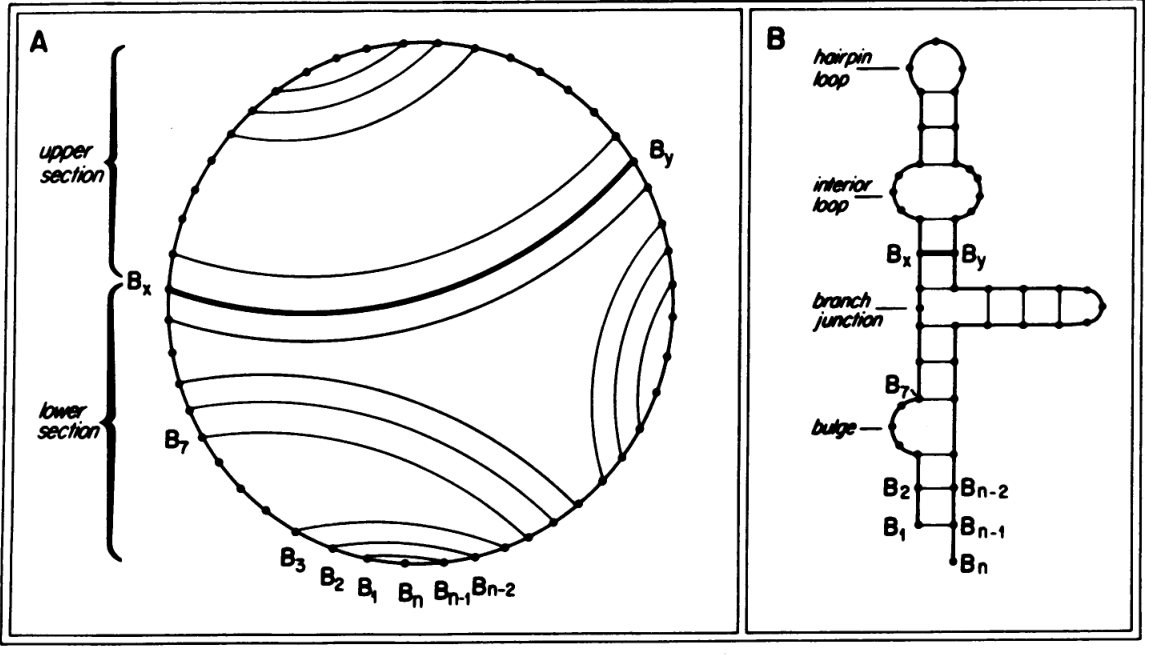
\includegraphics{figure1}}
\end{center}
\caption{RNA secondary structure as described in the Nussinov algorithm.
Taken from a publication by Nussinov \& Jacobson \cite{nussinov1980fast}.}
\label{figure1}
\end{figure}


Because of its dynamic programming nature, this algorithm performs recursive decompositions of the RNA and builds
larger structures out of repeated substructures. A natural representation of this is
depicted in Figure \ref{figure1}. Part A of Figure \ref{figure1} shows bonds as arcs across a circular
graph. In it, we see the nested nature of the structures being explored by the
Nussinov algorithm. Part B shows how these structures translate to actual RNAs,
and how these appear in vivo.

\begin{equation} \label{eq:nuss_eq}
	M(i, j) = \max \left\lbrace A, B, C, D \right\rbrace 
\end{equation}
\[
A = M(i, j-1)
\]
\[
B = M(i+1, j)
\]
\[
C = M(i+1, j-1) + W(i, j)
\]
\[
D = \max \left\lbrace M(i, k) + M(k+1, j) \right\rbrace \: when \: i < k < j
\]


In the recurrence relation show in Equation \ref{eq:nuss_eq} the first two cases ($A$ and $B$) find the score associated with not allowing $i$ and $j$ to bond. The case $C$ conversely determines the score given that $i$ and $j$ are bonded. The final case $D$ computes the score associated with a bifurcation. A bifurcation here means decomposition of the RNA into two separate structures between. This implies a $O(N^3)$
worst case time complexity and a $O(N^2)$ space complexity, as an $O(N^2)$ state space (all combinations of $i$ and $j$) is explored
with a linear time recurrence relation.



\section*{Circle Graphs and RNA}
A circle graph represents the intersection of a set of chords contained inside a circle.
A pair of chords $i, j$ and $k, l$ can be described in three ways. The pair is said to overlap if $i \leq k \leq j \leq l$. A chord $i, j$ is said to contain $k, l$ if $i < k < l < j$. Finally, the pair is said to be disjoint if the pair does not overlap, and if neither chord contains the other. A circle graph is obtained by transforming every chord into a node. Edges between nodes indicate overlapping chords (depicted in Figure \ref{circle2graph}). Such a graph can also be represented as a set of intervals on a line (depicted in Figure \ref{interval2circle}). This is geometrically equivalent to `cutting' the circle, and laying the line out in one dimension. Intuitively one can see that the potential bonds of an RNA molecule form such a graph. Indeed, circle graphs were used to depict RNA is Nussinov's original paper (see Figure \ref{figure1}) \cite{nussinov1980fast}.

\begin{figure}
\begin{center}
\scalebox{0.25}{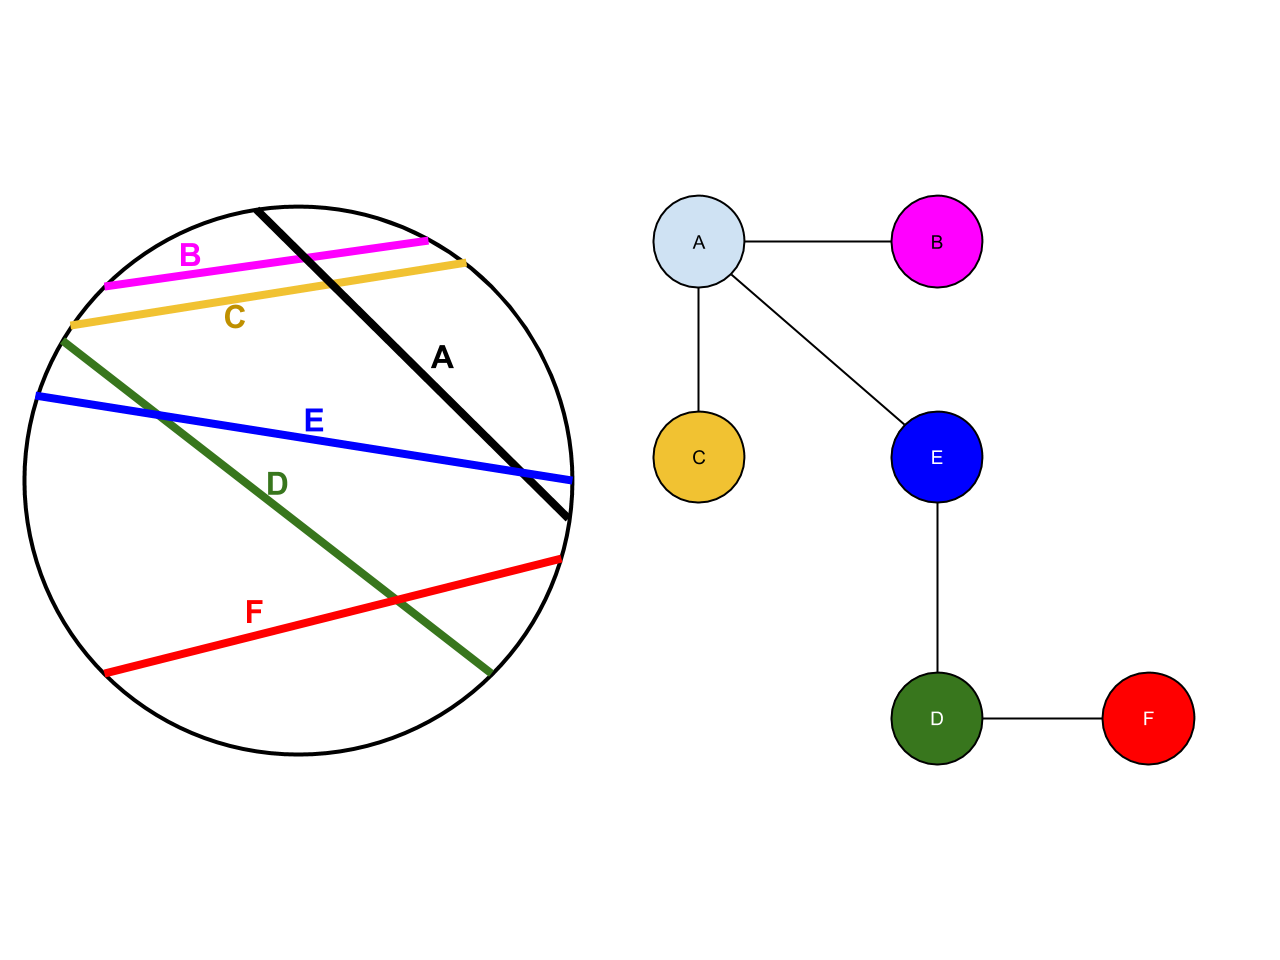
\includegraphics{circle2graph}}
\end{center}
\caption{The relationship between a chord model and a circle graph.}
\label{circle2graph}
\end{figure}


An independent set of a graph is a set of vertices which share no edges. Concordantly, it is a selection of chords which do not overlap. A maximum independent set is an independent set of maximum size---it contains the greatest possible number of vertices. If vertices are assigned weights, a maximum-weight independent set can also be computed, which is an independent set comprising vertices with maximum summed weight. Generally finding such sets is NP-Hard. However, in the case of circle graph, it can be solved in polynomial time. This is fortunate, as these algorithms have practical applications in register allocation \cite{de1999graph}, VLSI design \cite{cong1990over}, and bioinformatics \cite{swenson2009maximum}.

\begin{figure}
\begin{center}
\scalebox{0.25}{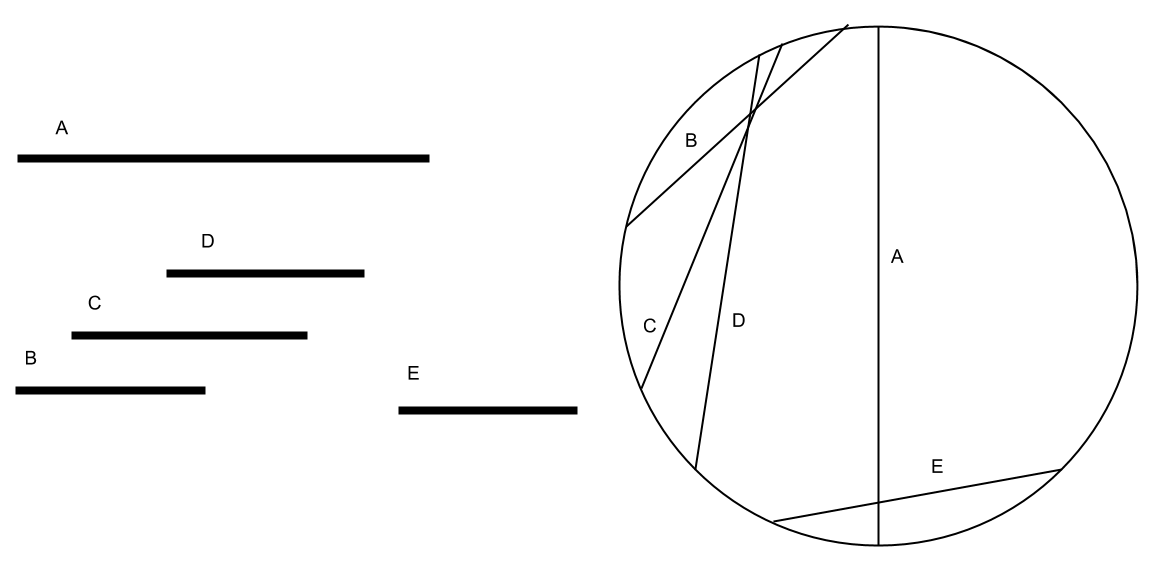
\includegraphics{interval2circle}}
\end{center}
\caption{The relationship between an interval model and a chord model.}
\label{interval2circle}
\end{figure}

The first algorithm for solving the maximum weight independent set of a circle graph was published in 1973 \cite{gavril1973algorithms}. It was able to find the set in $O(m^3)$ time and $O(m)$ space, where $m$ denotes the number of vertices in the circle graph. Later, in 2003, this bound was lowered by Valiente \cite{valiente2003new} who introduced an algorithm requiring $O(md)$ time. Here $d$ denotes the density of the graph. Density can be intuitively described as the maximum number of intervals crossing any point on the interval representation of a circle graph.  It also required $O(m)$ space, as do the following algorithms.

Bonsma \& Breuer \cite{bonsma2012counting} found an $O(nm)$ solution, where $n$ denotes the number of distinct end points for the chords in a circle graph. They noted that in dense graphs, where $m \geq n^2$, this algorithm is more optimal than the best known algorithms which take time $O(m^2)$. Shortly thereafter Nash \& Gregg \cite{nash2013new} presented an algorithm that computed the maximum-weight independent set of a circle graph using only $O(m + n\times \min \left\lbrace a^2, m\right\rbrace)$ time. Here $a$ denotes the independence number of the circle graph. The independence number of a graph is the cardinality of the largest independent set. In other words, it is the size of the maximum independent set. This is the best known algorithm to date.

The RNA folding algorithm first presented by Nussinov finds the maximum-weight independent set of a circle graph containing n endpoints in $O(m + n^3)$ where m is the total number of intervals or chords. In RNA there can never be two intervals with endpoints $i, j$ as a pair of endpoints uniquely identifies a bond. However, in the general case there may be many bonds with shared endpoints $i, j$, but with different weights. To solve the more general non-RNA case, we must first iterate over all the intervals, and for each $i, j$ index store the maximum-weight interval. This takes $O(m)$ time, as every interval is examined once, and the maximum-weight interval is stored in a 2D matrix whose indexes $i, j$ correspond to endpoints. The standard implementation of Nussinov’s algorithm can then be run with the W(i, j) function returning the value of the maximum-weight interval for endpoints $i, j$. Finally we are left with an algorithm that takes $O(m + n^3)$ time, and uses $O(n^2)$ space.


\section*{Conclusion}
It should be noted that the bound of $O(m + n^3)$ means that, when $a = n$ and $a^2 < m$ this algorithm is equivalent to that of Nash \& Gregg. And also that when $m \geq n^2$ it is more efficient than that of Bonsma \& Breuer. Furthermore it has better time complexity than Valentino's algorithm for any moderately dense graph, and is superior to the earlier algorithms which take $O(m^3)$ time, despite being first published in 1978, and it’s successor's current widespread use in bioinformatics to predict RNA secondary structure \cite{lorenz2011viennarna}. This is particularly surprising, since the maximum-weight independent set problem has often been concomitant with the use of RNA folding algorithms \cite{sperschneider2008knotseeker, bon2011tt2ne}.

Li, Ranka and Sahni \cite{li2013multicore} implemented the Nussinov algorithm on the GPU. This was reportedly up to 1582 times as fast as the single threaded version. They also outlined efficient multi-core implementations for the CPU, based on the same model.

For 25 year the Nussinov algorithm was the most optimal algorithm for finding the maximum weight independent set of a circle graph. Before 2013, it was still the most optimal algorithm in some cases. In addition, excellent parallel implementations of the Nussinov algorithm are available. Despite this, it was never recognised as finding, or used for finding, the maximum weight independent set for a circle graph. This starkly illustrates the problems inherent to cliquing within Science. I conjecture that this situation would have been avoided with a more holistic approach to research. All knowledge is valuable; insular research has no place in the advancement of Science.


\bibliographystyle{plain}
\bibliography{assignment_one}


\end{document}

